\documentclass[5pt]{article}
\usepackage{mathptmx,amsmath}
\usepackage{pdfslide2,pause}
\usepackage{eurosym}
\usepackage[portuguese,english]{babel}
\usepackage{kerkis}
\usepackage{colortbl} % used to highlight row or columns of tables. http://www.tug.org/pracjourn/2007-1/mori/mori.pdf
\usepackage[small]{caption} % more option on http://www.dd.chalmers.se/latex/Docs/PDF/caption.pdf
\usepackage[tight,scriptsize]{subfigure}
\usepackage{lastpage}
\usepackage{chngcntr}
\usepackage[absolute,overlay]{textpos}
\usepackage{tabto}
\usepackage{animate}

\usepackage{multicol}
\usepackage{tcolorbox}
\usepackage{booktabs}

\usepackage{hyperref}
\hypersetup{
	colorlinks=true,
	linkcolor=blue,
	filecolor=magenta,      
	urlcolor=cyan,
}


%\usepackage{listings}
\captionsetup{labelformat=empty,skip=-0.8cm}

%\lstset{
%    language=Matlab,                % choose the language of the code
%    basicstyle=\ttfamily\tiny,       % the size of the fonts that are used for the code
%    numbers=none,                   % where to put the line-numbers
%    numberstyle=\tiny,              % the size of the fonts that are used for the line-numbers
%    stepnumber=1,                   % the step between two line-numbers. If it's 1 each line will be numbered
%    numbersep=5pt,                  % how far the line-numbers are from the code
%    backgroundcolor=\color{white},  % choose the background color. You must add \usepackage{color}
%    showspaces=false,               % show spaces adding particular underscores
%    showstringspaces=false,         % underline spaces within strings
%    showtabs=false,                 % show tabs within strings adding particular underscores
%    tab=\rightarrowfill,
%    frame=none,	                 % adds a frame around the code
%    tabsize=2,	                   	 % sets default tabsize to 2 spaces
%    captionpos=b,                   % sets the caption-position to bottom
%    breaklines=true,                % sets automatic line breaking
%    breakatwhitespace=false,        % sets if automatic breaks should only happen at whitespace
%    title=\lstname,                 % show the filename of files included with \lstinputlisting; also try caption instead of title
%    escapeinside={\%*}{*)},          % if you want to add a comment within your code
%    morekeywords={ifftshift,fftshift},
%    keywordstyle=\bfseries\color[rgb]{0,0,0.3},
%    commentstyle=\color[rgb]{0.133,0.5,0.133}
%}
%\lstset{
%    emph={function,end,for,if,while},
%    emphstyle=\bfseries\color[rgb]{0.6,0,0},
%}

\definecolor{itblue}{rgb}{0.0,0.0,0.5}
\definecolor{itred}{rgb}{0.82,0.18,0.24}
\newcommand{\pageNum}{
    \begin{picture}(0,0)(0,0)
        \put(-15,-390){
            \begin{minipage}{1.8cm}
            \end{minipage}
        }
    \end{picture}
}
\newcommand{\cb}[1]{{\color{itblue} #1}}%
\newcommand{\cred}[1]{{\color{itred} #1}}%
\newcommand{\bb}[1]{{\textbf{\color{itblue} #1}}}%
\newcommand{\br}[1]{{\textbf{\color{itred} #1}}}%
\renewcommand{\labelitemi}{\textcolor{itred}{\normalsize $\bullet$}}
\renewcommand{\labelitemii}{\textcolor{itblue}{$\bullet$}}
\newcommand{\mysection}[1]{\section*{\pageNum\color{itred}\sffamily #1}\vspace*{0.5cm}\overlay{it_1.png}\sffamily}%
\newcommand{\ITfootnote}[1]{\hspace{1.8cm}\begin{minipage}{13cm}\tiny{#1}\end{minipage}}
\newcommand{\edfaGain}{$G=\exp\left(\frac{\alpha}{2}L_{span}\right)$}
\newenvironment{reference}{
    \begin{textblock*}{0.7\textwidth}(32mm,137mm)\tiny\noindent\bgroup\color{black}
}
{
    \egroup\end{textblock*}
}


\graphicspath{{./Figures/}}
\pagestyle{title}

\hyphenpenalty=50000
\tolerance=10000

\setlength{\textheight}{1.5\textheight}

%%%%%%%%%%%%%%%%%%%%%%%%%%%%%%%%%%%%%%%%%%%%%%%%%%%%%%%%%%%%%%%%%%%%%%%%%%%%%%%%%%%%%%%%%%%%%%%%%%%
%%%%%%%%%%%%%%%%%%%%%%%%%%%%%%%%%%%%%%%%%%%%%%%%%%%%%%%%%%%%%%%%%%%%%%%%%%%%%%%%%%%%%%%%%%%%%%%%%%%

\begin{document}

%************************************************************************************************
%                                          SLIDE
%************************************************************************************************
\pagenumbering{roman}
\begin{titlepage}  \overlay{it_0.png}

\color{itblue} \sffamily \noindent \small
\hspace*{1cm}  Universidade de Aveiro\\ %Instituto\\ Superior T�cnico, Instituto de Telecomunica��es\\
\hspace*{1cm}  2017-2018\\ %Lisboa, 14th of February, 2013\\

\vspace*{1cm}
\begin{center}
    \color{black} \sffamily \noindent \Large
    \br{Introduction to the software Net2plan\\}
\end{center}
\vspace{6mm}
\begin{center}
    \color{black}
    \textbf{Romil Patel\\}
    {(romilkumar@ua.pt)}
\end{center}

\vspace{0.0mm}
\scriptsize
\begin{center}
Department of Electronics, Telecommunications and Informatics,\\
University of Aveiro, Aveiro, Portugal\\
Instituto de Telecomunica\c{c}\~{o}es, Aveiro, Portugal\\
\end{center}

\vspace{1.0cm}
\hspace*{13.2cm}\tiny \copyright 2005, it - instituto de telecomunica\c{c}\~{o}es\hfill

\end{titlepage}


\renewcommand{\headsep}{-25pt}
\pagenumbering{arabic}



%--------------------------------------------------------------------------------------------------
%------------ SLIDE-------
\mysection{Net2Plan download and installation}\large
\vspace{0cm}

\begin{itemize}
  %\item Coherent optical transmission schemes are optimal from the stand point of spectral efficiency since they allow the encoding of information in both quadrature and polarization.
  
    \item \textbf{Step 1 :} Since Net2plan coded in Java, first step is to make sure that computer has necessary \textbf{Java Runtime Environment}. This can be downloaded from \textbf{\url{https://java.com/en/download/}} and install it in your computer.
	\item \textbf{Step 2 :} Next download \& install Net2plan software. Net2plan is available on \textbf{\url{http://net2plan.com/download.php}}.
	\begin{itemize}
		\item There are several versions available on the website, however, please download a stable version "net2plan-0.4.2.zip".
		\item Extract it and find the \underline{executable jar file} with the name of "Net2Plan".
		\item Double click on it and it'll open the following window (see next page):
	\end{itemize}
\end{itemize}
\
%--------------------------------------------------------------------------------------------------
%------------ SLIDE-------
\mysection{}\large

\begin{figure}[hbt]
	\centering
	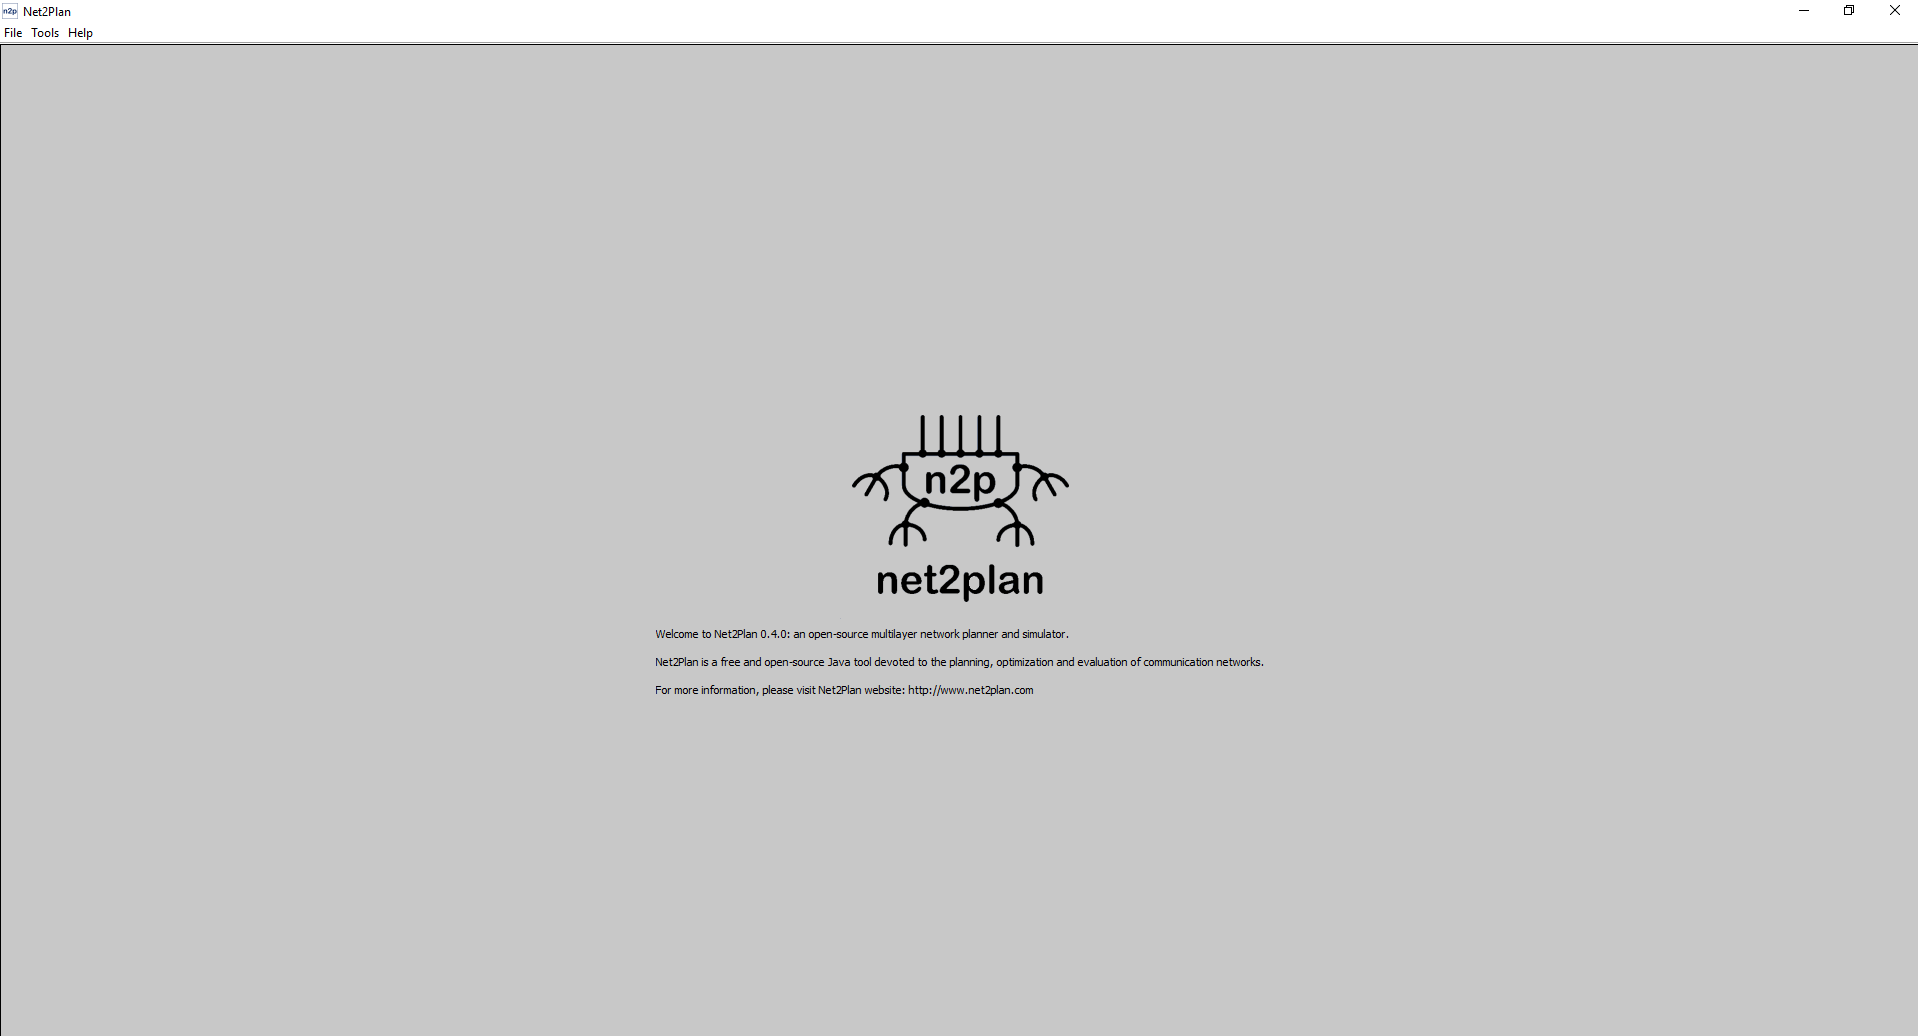
\includegraphics[width=0.8\textwidth, height=8cm]{./figures/2.png}
    \vspace{10mm}
    \caption{}\label{}
\end{figure}

Now we have Net2plan software installed in our computer !!!

%--------------------------------------------------------------------------------------------------
%------------ SLIDE-------
\mysection{Net2plan Tools}\large
\begin{itemize}
	\item \textbf{Creating Traffic Matrices : }\\
	\textbf{Step 1 :} To start creating a traffic matrix in Net2Plan go to "Tools $\rightarrow$ Traffic matrix design" or press "Alt +2".
	This will pop-up the following window:
\begin{figure}[hbt]
	\centering
	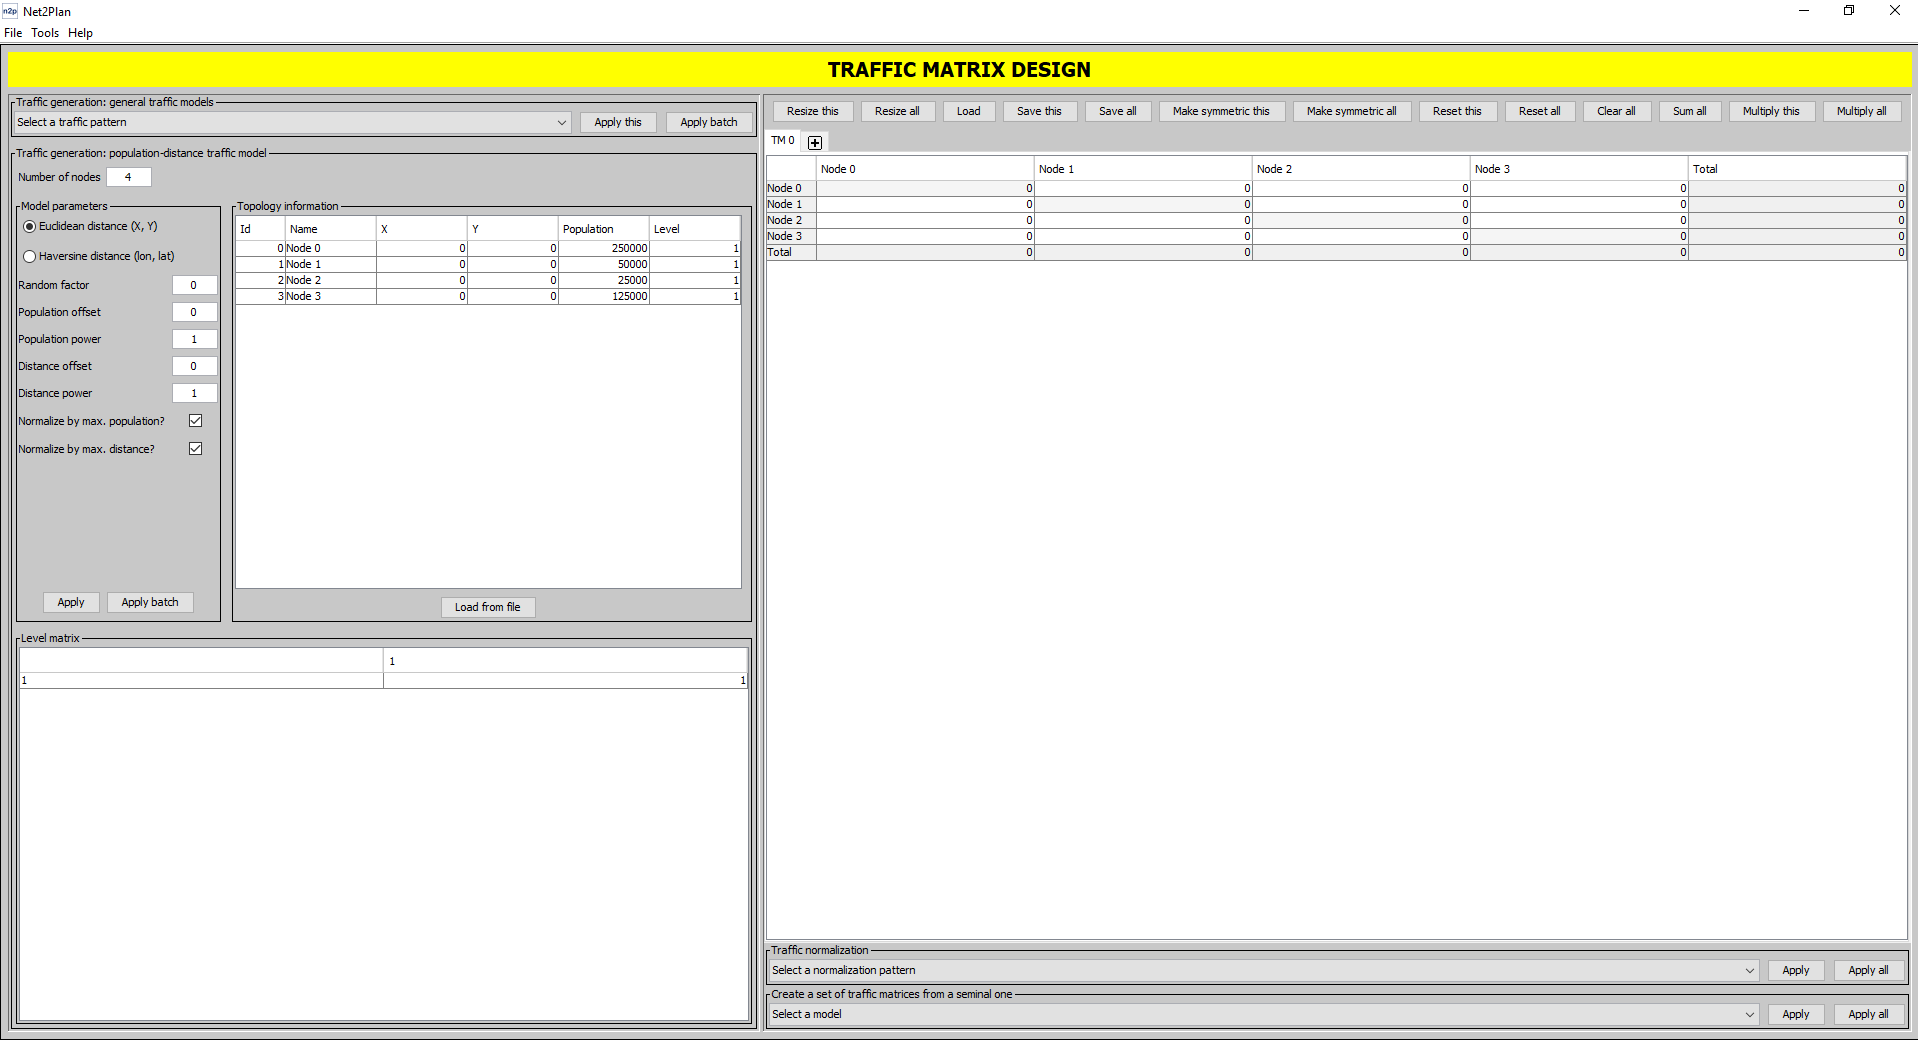
\includegraphics[width=0.8\textwidth, height=8cm]{./figures/4.png}
	\vspace{10mm}
	\caption{}\label{}
\end{figure}
\end{itemize}


%--------------------------------------------------------------------------------------------------
%------------ SLIDE-------
\mysection{}\large
\vspace{0cm}
\begin{itemize}
	\item \textbf{Step 2 :} Click on the top left side "select a traffic pattern". This will open a palate which includes several types of option for traffic pattern. From these options, select "Constant" (see the following figure). 
\begin{figure}[hbt]
	\centering
	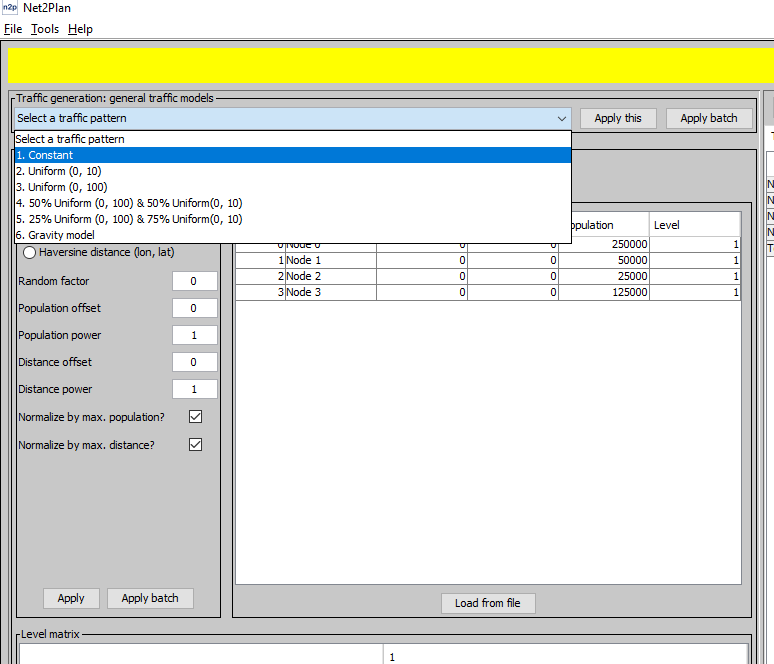
\includegraphics[width=0.8\textwidth, height=8cm]{./figures/5.png}
	\vspace{8mm}
	\caption{}\label{}
\end{figure}
\end{itemize}
%--------------------------------------------------------------------------------------------------
%------------ SLIDE-------
\mysection{}\large
\vspace{0cm}
\begin{itemize}
	\item \textbf{Step 3 :} Next we'll create batch of matrices with constant traffic. for that click "Apply batch". This will pop-up a new box (see the figure) and fill all the value as per the following:\\
	Number of nodes$\rightarrow$ 6\\
	Number of matrices $\rightarrow$ 5\\
	Constant value $\rightarrow$ 1\\
\begin{figure}[hbt]
	\centering
	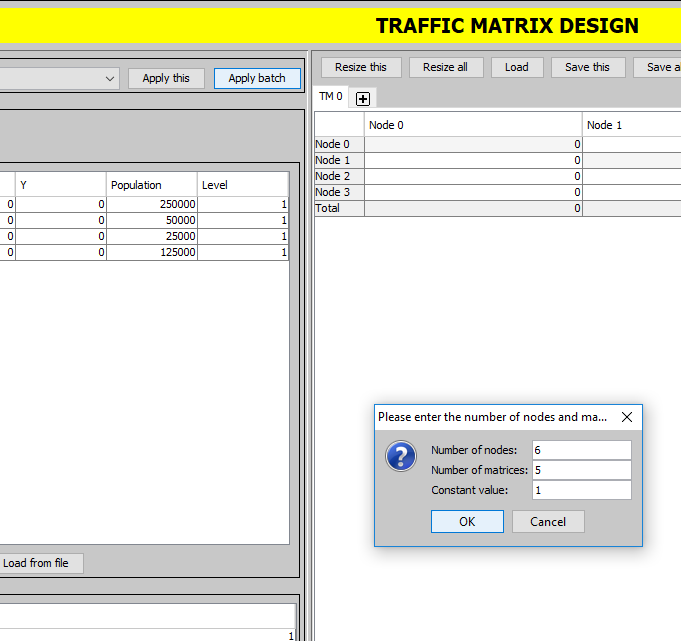
\includegraphics[width=0.4\textwidth, height=5cm]{./figures/6.png}
	\vspace{8mm}
	\caption{}\label{}
\end{figure}
\end{itemize}
%--------------------------------------------------------------------------------------------------
%------------ SLIDE-------
\mysection{}\large
\begin{itemize}
	\item \textbf{Step 4 :} This will create 5 different matrices. Now update the value of all the matrices according to your ODU matrices (To edit its value, double click on it).\\
Next click on "Save all" to save all these matrices.
\begin{figure}[hbt]
	\centering
	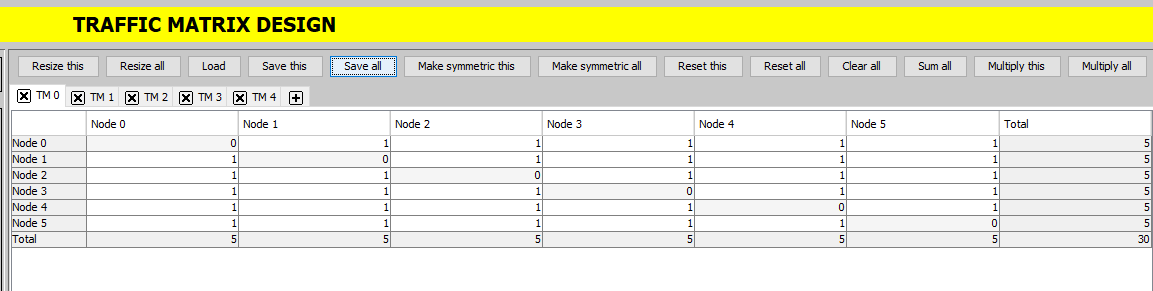
\includegraphics[width=0.9\textwidth, height=6cm]{./figures/7.png}
	\vspace{8mm}
	\caption{}\label{}
\end{figure}
\end{itemize}
%-------------------------------------------------------------------
%------------ SLIDE ------------------------------------------------
\mysection{}\large
\begin{itemize}
	\item \textbf{Creating the Network topologies : }\\
	\textbf{Step 1 :} To start the network creation in Net2plan go to "Tools $\rightarrow$ Offline network design" or press "Alt +1". This will pop-up the following window:
	\begin{figure}[hbt]
		\centering
		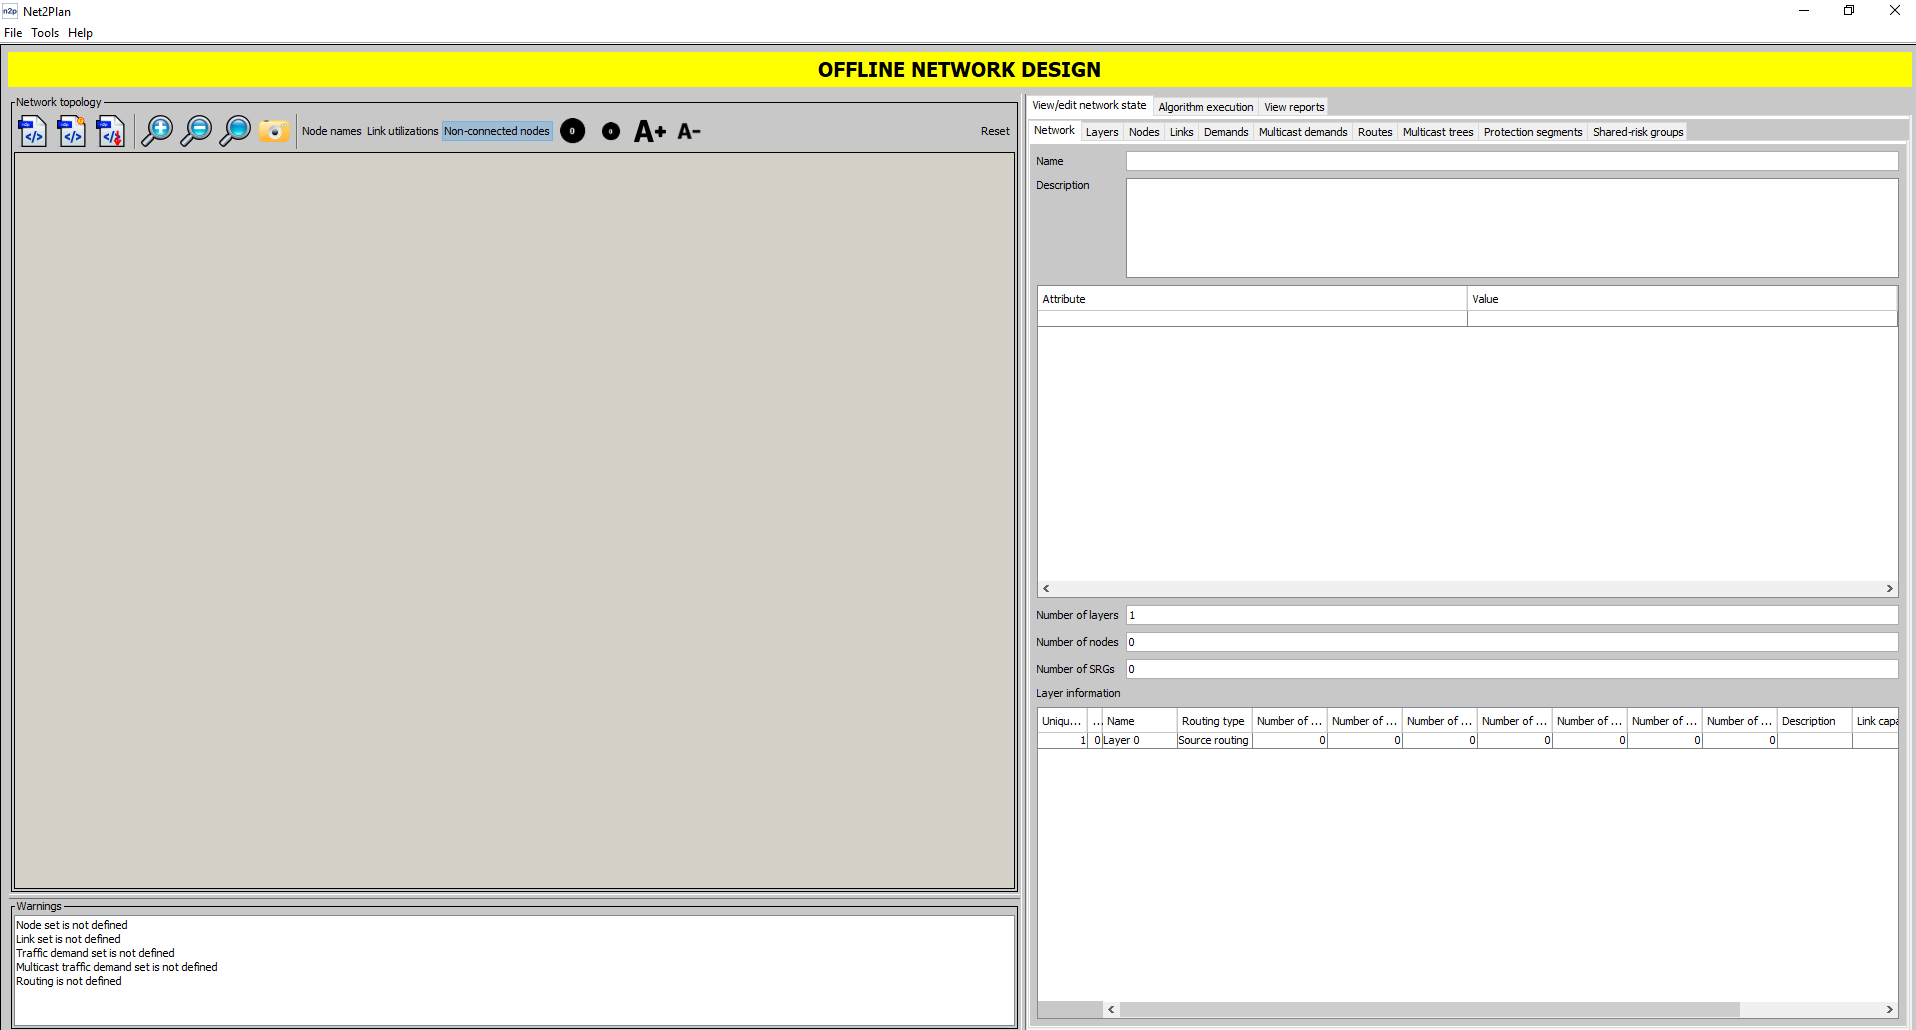
\includegraphics[width=0.8\textwidth, height=8cm]{./figures/8.png}
		\vspace{8mm}
		\caption{}\label{}
	\end{figure}
\end{itemize}
%-------------------------------------------------------------------
%------------ SLIDE ------------------------------------------------
\mysection{}\large
\begin{itemize}
	\item \textbf{Step 2 :} To start creating a new network, first nodes have to be introduced by right clicking on the gray area and choosing "Add node here".
	\begin{itemize}
	\item Links between nodes are created by holding a click on the origin node and dragging until the destination node, holding shift before releasing the click creates bidirectional links.
	\item Create a full network as shown in figure.
	\begin{figure}[hbt]
	\centering
	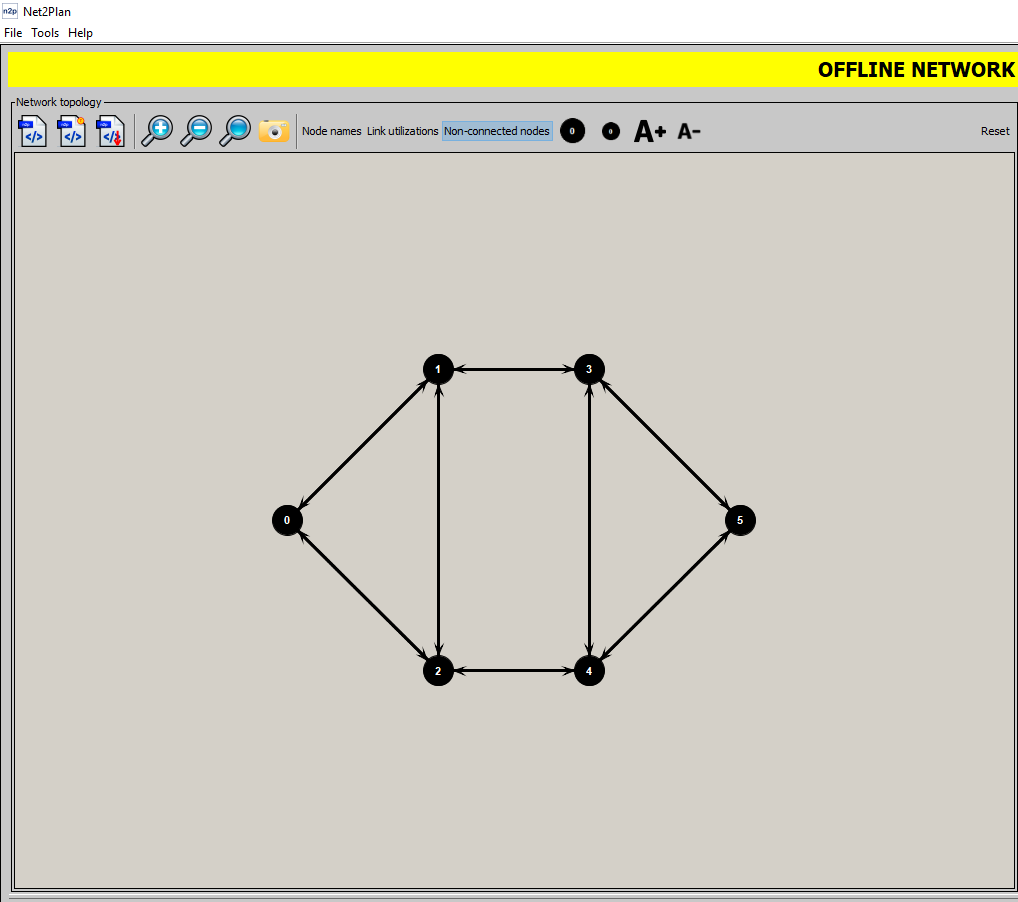
\includegraphics[width=0.6\textwidth, height=6cm]{./figures/9.png}
	\vspace{8mm}
	\caption{}\label{}
\end{figure}
\end{itemize}
\end{itemize}

%-------------------------------------------------------------------
%------------ SLIDE ------------------------------------------------
\mysection{}\large
\begin{itemize}
	\item \textbf{Step 3 : } View/edit network states\\ 
It displays all the characteristics/states of our network. Modify it where where applicable (i.e. in "links", we can set the capacity of the each link.) 
		\begin{figure}[hbt]
			\centering
			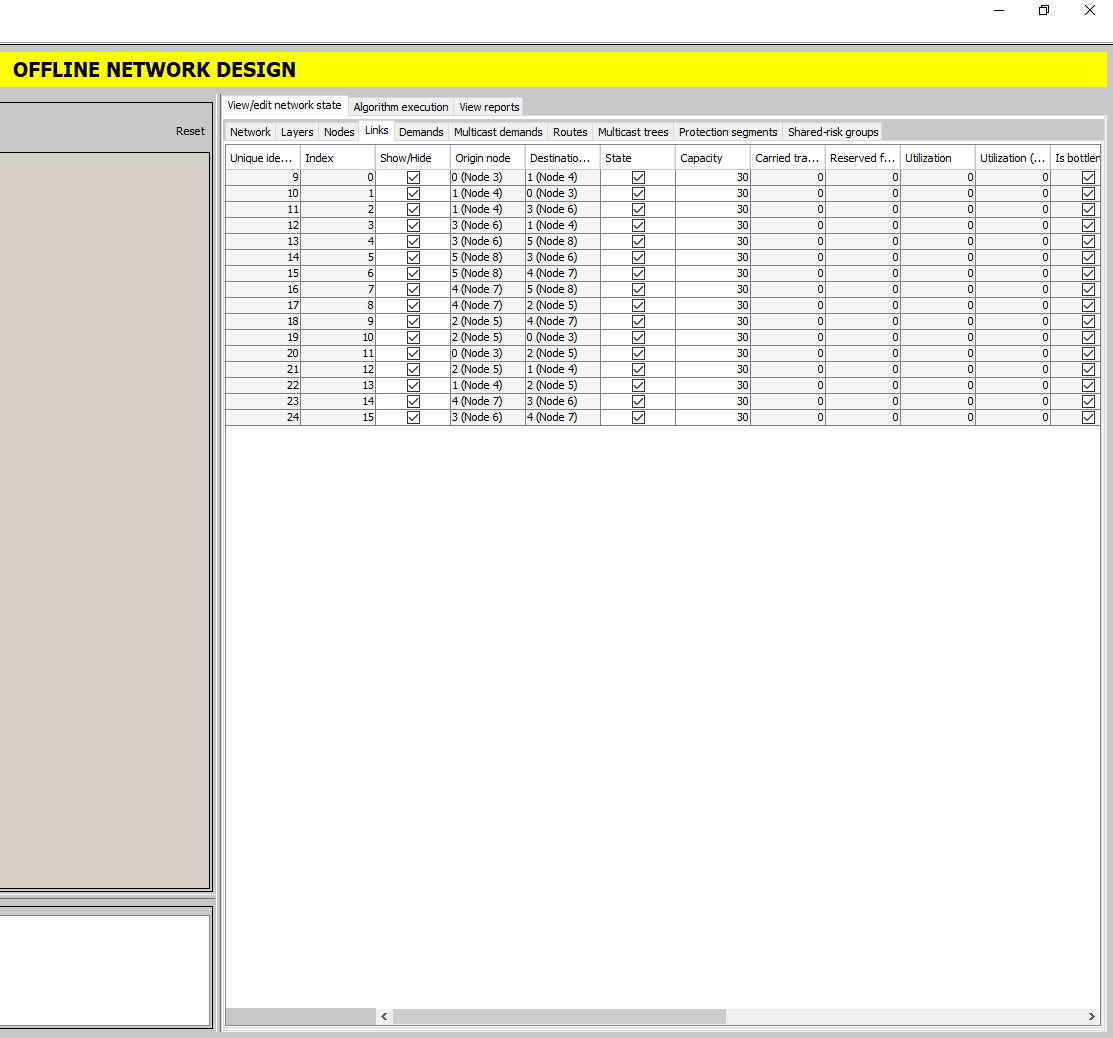
\includegraphics[width=0.8\textwidth, height=8cm]{./figures/10.png}
			\vspace{8mm}
			\caption{}\label{}
		\end{figure}
\end{itemize}
%-------------------------------------------------------------------
%------------ SLIDE ------------------------------------------------

\mysection{}\large
\begin{itemize}
	\item \textbf{Step 4 : } Algorithm execution
	\begin{itemize}
	\item Set the path of the algorithm (i.e. C:/Net2plan-0.4.2/NetPlanner\_vb.jar). This includes three different algorithm :\\
	 1. joinTrafficMatricies\\
	 2. logicalTopology\\
	 2. Grooming\_dedicated
	
	
		
	\begin{figure}[hbt]
		\centering
		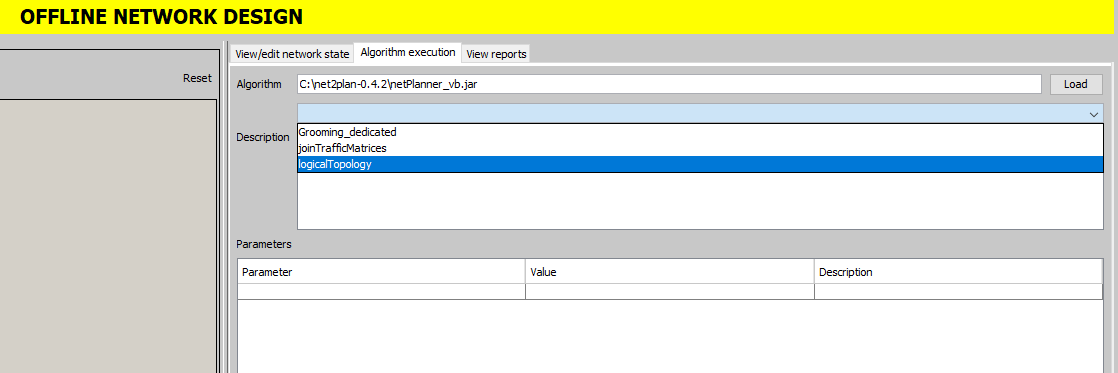
\includegraphics[width=0.7\textwidth, height=5cm]{./figures/11.png}
		\vspace{8mm}
		\caption{}\label{}
	\end{figure}
\end{itemize}
\end{itemize}
%-------------------------------------------------------------------
%------------ SLIDE ------------------------------------------------
\mysection{}\large
\begin{itemize}
	\item \textbf{Step 5 : } From the palate, first select "jonTrafficMatricies".\\
	Now set the path of the all ODU matrices which we have created earlier. (i.e. C:\textbackslash net2plan-0.4.2/workspace/data/trafficMatrices/ODU0.n2p )
		\begin{figure}[hbt]
			\centering
			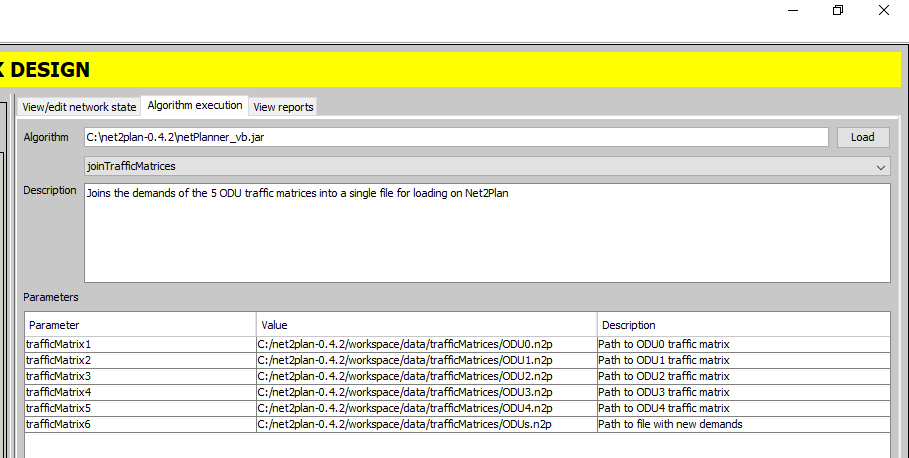
\includegraphics[width=0.7\textwidth, height=5cm]{./figures/12.png}
			\vspace{8mm}
			\caption{}\label{}
		\end{figure}
	\end{itemize}

After setting all path of ODUs, click on the "Execute" buttons.
%-------------------------------------------------------------------
%------------ SLIDE ------------------------------------------------
\mysection{}\large
\begin{itemize}
	\item \textbf{Step 6 : } From the palate, select "logicalTopology".\\
	Read the description in the Net2plan to understand the function of the algorithm.
	\begin{figure}[hbt]
		\centering
		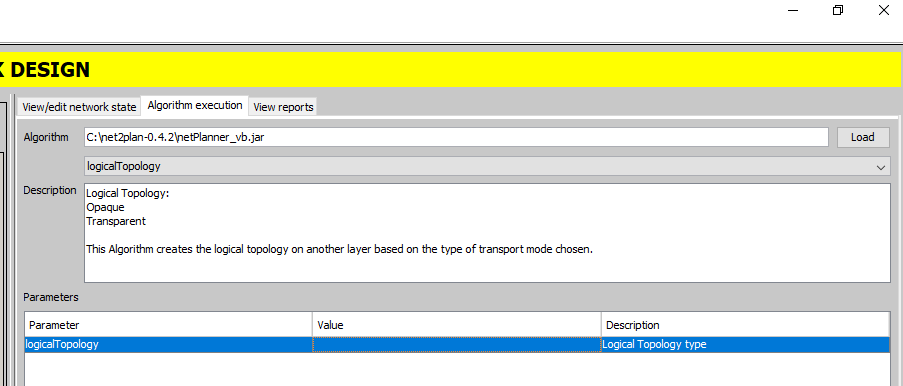
\includegraphics[width=0.7\textwidth, height=5cm]{./figures/13.png}
		\vspace{8mm}
		\caption{}\label{}
	\end{figure}
\end{itemize}

click on the "Execute" buttons.
%-------------------------------------------------------------------
%------------ SLIDE ------------------------------------------------
\mysection{}\large
\begin{itemize}
	\item \textbf{Step 7 : } From the palate, select "Grooming\_dedicated".\\
		Read the description in the Net2plan to understand the function of the algorithm.
	\begin{figure}[hbt]
		\centering
		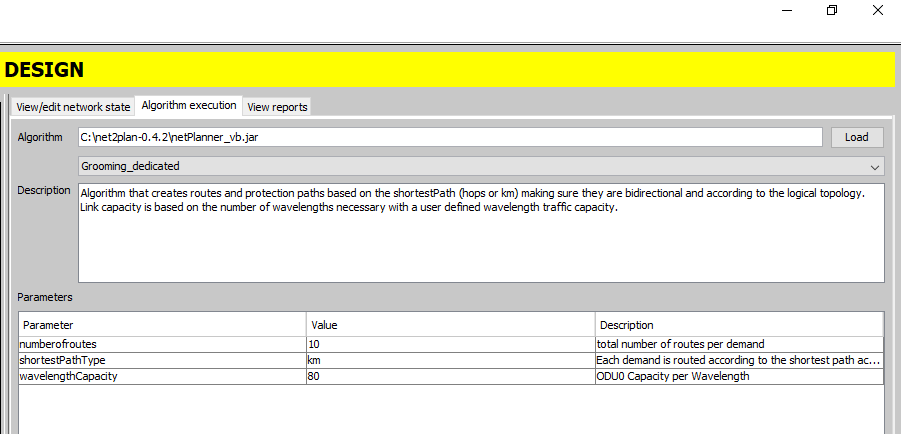
\includegraphics[width=0.7\textwidth, height=5cm]{./figures/14.png}
		\vspace{8mm}
		\caption{}\label{}
	\end{figure}
\end{itemize}

click on the "Execute" buttons.
%-------------------------------------------------------------------
%------------ SLIDE ------------------------------------------------
\mysection{}\large
\begin{itemize}
\item  \textbf{View Reports : }\\
This section will generate a table which includes number of optical channels, ports and calculates the network cost.
	\begin{figure}[hbt]
		\centering
		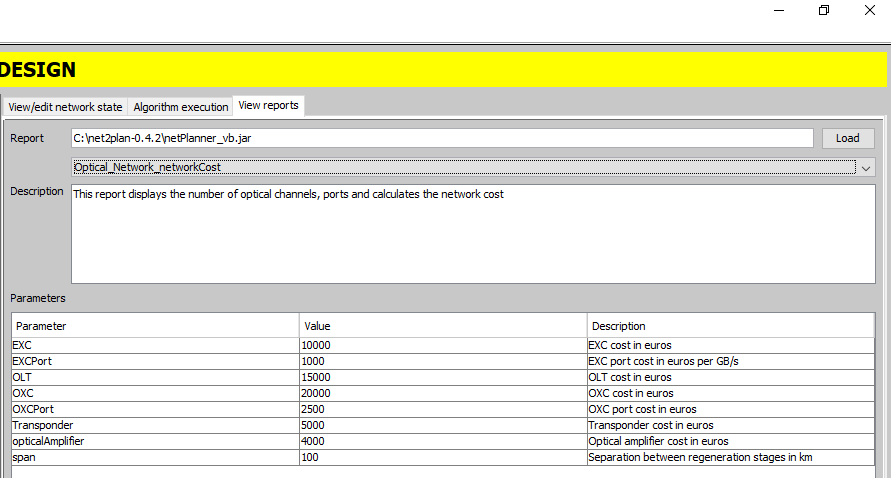
\includegraphics[width=0.8\textwidth, height=8cm]{./figures/15.png}
		\vspace{10mm}
		\caption{}\label{}
	\end{figure}
\end{itemize}

%-------------------------------------------------------------------
%------------ SLIDE ------------------------------------------------

\mysection{} \sffamily
\vspace{-10mm}
\large\centerline{E-mail: romilkumar@ua.pt}


\end{document}
